\documentclass[12pt,a4paper]{article}
\usepackage{kotex}
\usepackage{graphicx}
\usepackage{hyperref}
\usepackage{indentfirst}
\usepackage{subcaption}
\usepackage{multirow}
\usepackage{flafter}
\usepackage{tikz}
\usepackage{wrapfig}
\usepackage{spreadtab}
\usetikzlibrary{arrows.meta, intersections, decorations.markings,
    positioning, backgrounds, through, calc, angles, quotes}
\setlength{\parskip}{2mm}
\usepackage{amsmath}
\usepackage[top=3cm, bottom=2.54cm, left=2.54cm, right=2.54cm]{geometry}
\usepackage[yyyymmdd]{datetime}
\renewcommand{\dateseparator}{-}
\usepackage{array}
\newcolumntype{L}[1]{>{\raggedright\let\newline\\\arraybackslash\hspace{0pt}}m{#1}}
\newcolumntype{C}[1]{>{\centering\let\newline\\\arraybackslash\hspace{0pt}}m{#1}}
\newcolumntype{R}[1]{>{\raggedleft\let\newline\\\arraybackslash\hspace{0pt}}m{#1}}

\begin{document}
\begin{titlepage}
    \centering
    \begin{tabular}{|C{15cm}|}
        \hline
        \rule{0in}{6ex}
        {\huge 물리학 및 실험 1\par} \\ 
        {\large 힘센서를 활용한 충격량과 작용 반작용 법칙\par} \\
        \hline
    \end{tabular} \\
    \vspace{5cm}
    
\includegraphics[height=7.36cm]{logo.png}\par
    \vspace{3cm}
    \begin{tabular}{|l|l|l|l|l|l|}
        \hline
        과목 & \multicolumn{5}{l|}{물리학및실험1} \\
        \hline
        담당교수 & \multicolumn{2}{l|}{전계진} & 담당조교 & \multicolumn{2}{l|}{} \\
        \hline
        조 및 조원 & \multicolumn{5}{l|}{2조, 김민수 김민규 김민서 김백준 김연주} \\
        \hline
        제출일 & \multicolumn{5}{l|}{\today} \\
        \hline
        작성자 & 김민수 & 학번 & 20518009 & 학과 & 정보보호 \\
        \hline
    \end{tabular}
\end{titlepage}
\section{실험목적}
\begin{itemize}
    \item 스마트 카트를 이용하여 충돌실험을 하고 충돌 전후에 카트의 운동량 변화가
        카트가 받는 충격량과 같은지 확인한다.
    \item 충돌하는 두 물체 사이에 작용하는 힘이 작용반작용의 법칙을 따르는지
        확인한다.
\end{itemize}
\section{서론}
\begin{itemize}
    \item 일상에서 물체가 충돌하는 일은 자주 발생한다. 두 물체가 서로 충돌할 때 매우
        짧은 시간 동안 순간적으로 큰 힘이 작용한다. 이 때문에 뉴턴의 운동 제2 법칙으
        로 이러한 현상을 설명하기는 쉽지 않다.
    \item 물리학에서는 이와 같은 충돌 현상을 설명하기 위해 운동량과 충격량 개념을 도
        입한다. 충돌이나 폭발과 같은 현상에서도 총운동량이 보존되고 각각의 물체가
        받은 충격량은 자신의 운동량 변화와 같다는 충격량-운동량 정리가 성립한다고
        알려져 있다.
    \item 우리는 힘 센서와 스마트 카트를 이용하여 물체가 서로 충돌하는 실험을 하고,
        충돌하는 두 물체 사이에 작용반작용의 법칙과 충격량-운동량 정리가 성립하는가
        를 알아볼 것이다.
    \item 힘 센서를 이용하여 충돌하는 두 물체 사이에 작용하는 힘을 측정하여 뉴턴의
        운동 제3 법칙인 작용반작용의 법칙이 성립하는가를 확인하고, 스마트 카트에
        내장된 속도 센서로 속도를 측정하여 충격량-운동량 정리가 성립하는가를 알아볼
        것이다.
\end{itemize}
\section{실험원리}
\subsection{운동량 및 운동량과 힘과의 관계}
운동량은 벡터 $\vec{p}$로 나타내며 질량과 속도의 곱으로 정의 한다.
$$\vec{p}=m\vec{v}$$
뉴턴의 제2법칙 “운동량의 시간변화율은 알짜 힘과 같다”
$$\Sigma\vec{F}=\frac{\Delta\vec{v}}{\Delta t} =
    \frac{\Delta m}{\Delta t}\vec{v}+m\frac{\Delta\vec{v}}{\Delta t} = 
    \frac{\Delta m}{\Delta t}\vec{v}+m\vec{a}$$
질량이 일정한 경우 $\Sigma\vec{F}=m\vec{a}$
\subsection{운동량 충격량 정리}
충돌하는 동안에는 물체에 큰 힘이 작용하여 물체가 변형이 된다.
$$\Sigma\vec{F}=\frac{d\vec{p}}{dt} \Rightarrow
    d\vec{p} = \Sigma\vec{F}dt \Rightarrow
    \Delta\vec{p} = \vec{p}_2 - \vec{p}_1 = \int^{t_2}_{t_1}\Sigma\vec{F}dt$$
충격량(Impulse): 물체가 받는 충격의 정도를 나타냄
\begin{figure}[h!]
    \centering
    \begin{subfigure}{0.3\textwidth}
        $\vec{I}\equiv\int^{t_f}_{t_i}\Sigma\vec{F}dt$ \\
        $\Delta\vec{p}=\vec{p}_2-\vec{p}_1=\vec{I}$
    \end{subfigure}
    \begin{subfigure}{0.3\textwidth}
        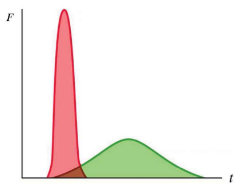
\includegraphics[height=3.36cm]{W11G1.png}
    \end{subfigure}
    \begin{subfigure}{0.3\textwidth}
        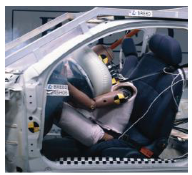
\includegraphics[height=3.36cm]{W11G2.png}
    \end{subfigure}
\end{figure}
충격량-운동량 정리
\begin{enumerate}
    \item 충돌 이전의 속력과 이후의 속력을 이용하여:
        $\Delta\vec{p}=\vec{p}_2-\vec{p}_1$
    \item 충돌 중 시간에 따른 힘의 변화를 이용하여:
        $\vec{I}\equiv\int^{t_f}_{t_i}\Sigma\vec{F}dt=F_{avg}\Delta t=
        \Delta\vec{p}$
\end{enumerate}
\begin{figure}[h!]
    \centering
    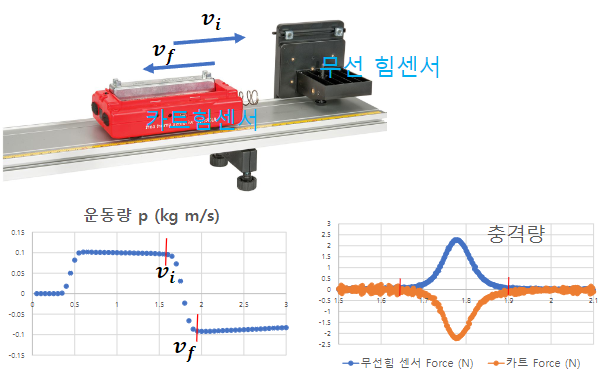
\includegraphics[width=15cm]{W11G3.png}
\end{figure}
\subsection{작용 반작용의 법칙}
\begin{wrapfigure}{l}{5.1cm}
    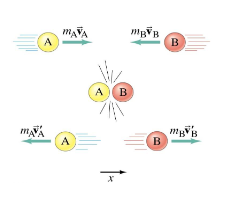
\includegraphics[width=5cm]{W11G4.png}
\end{wrapfigure}
“관성 기준틀에서, 첫번째 물체가 두번째 물체에 힘을 작용할 때마다 (동시에) 두번째
물체는 첫 번째 물체에 크기는 같고 방향이 반대인 힘을 작용한다”

= 작용 반작용의 법칙

$\vec{F}_12=-\vec{F}_21$
\clearpage
\section{실험기구 및 장치}
\begin{itemize}
    \item 역학트랙, 힘 센서 브라켓, 자기 범퍼, 스프링 범퍼 2개, 스텐드. 수평계,
        500g 쇠막대
    \item 센서 실험장치: data 수집 및 분석 software (Capstone), 스마트 카트,
        무선힘센서
\end{itemize}
\begin{figure}[h!]
    \centering
    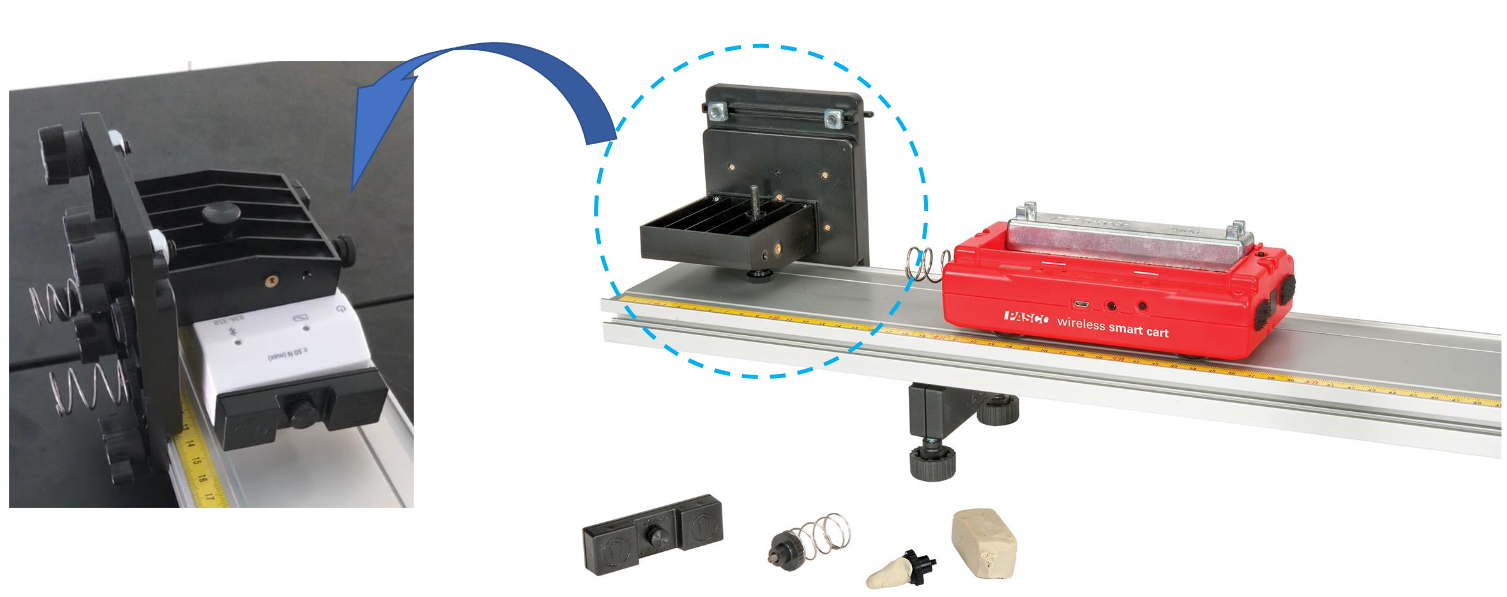
\includegraphics[width=15cm]{W11G5.png}
\end{figure}
\section{실험방법}
트랙의 끝에 힘센서를 고정하고 스마트 카트와 충돌할때 충격량과 카트의 운동량 변화를
측정하고, 탄성을 다르게 했을 때와 비교하고 작용 반작용 법칙을 확인한다.
\begin{itemize}
    \item [준비1] \begin{enumerate}
            \item 역학 트랙을 설치하고 한쪽 끝에는 자기범퍼, 다른 한쪽에는
                힘센서 브라켓을 설치한다.
            \item 힘센서 브라켓에 무선 힘센서를 설치하고 센서 앞부분에 자기범퍼를
                설치한다.
            \item Smart Cart에도 자석 범퍼를 장착한다.
            \item 트랙위에 수평계를 올려놓고 좌우 수평을 맞춘다.
        \end{enumerate}
    \item [준비2] \begin{enumerate}
            \item 캡스톤 실행
            \item 스마트카트 연결하고 내장된 센서 (위치, 속도, 가속도, 힘센서)를
                설정한다(힘센서는[change sign]을 체크한다, 당기는 힘을 음으로
                출력하기 때문. 카트의 힘을 음의 힘으로 출력하기 위함이다)
            \item 무선힘센서가 연결된 것을 확인한다.
            \item 캡스톤의 Calculator에서 운동량 (p=mv)를 선언한다. ※카트추의
                질량을 바꿀 때마다 m값 변경※
            \item 표와 그래프 모드로 선택하여 표의 칼럼을 추가하여 시간, 속도,
                힘(카트), 힘(무선힘센서)을 설정하고 그래프에도 그래프를 추가하여
                힘-시간, P(운동량)-시간 축을 설정하고 힘은 힘(카트), 힘(무선힘센서)
                를 모두 설정하고, sample rate를 200Hz로 설정한다.
        \end{enumerate}
\end{itemize}
\clearpage
\begin{itemize}
    \item [실험1.] 운동량 충격량 측정(자기적 반발력 이용)
        \begin{enumerate}
            \item 데이터 기록하기 전 힘 센서 윗면의 tare 버턴을 눌러 0점 조절한다.
                (매 측정 마다 한다)
            \item 스마트 카트의 힘센서도 화면 아랫쪽의 카트 힘센서를 선택하여
                영점조절 버턴을 누른다. (매 측정 마다 한다)
            \item 카트, 추 질량 측정하고 기록한다.
            \item {\label{it:4} Smart Cart의 플런저를 1단으로 맞춘 후
                End Stop앞에 정지시킨다.}
            \item 카트에 추(500g)을 싣고 방아쇠를 눌러 카트를
                출발시킨 후 Force Sensor와 충돌 후 운동방향이 바뀔 때까지 과정을
                Capstone으로 측정 후 충격량과 운동량의 변화를 비교해본다.
            \item 시간-운동량의 그래프를 확인한다.
            \item 그래프에서 smart tool 버턴을 눌러 충돌전 운동량과 그때의 시간 및
                충돌후 운동량과 그때 시간을 데이터 표에 기록한다. 그래프를 같이
                첨부해서 제출한다.
            \item 시간-힘의 그래프에서 충격량을 구한다.
            \item {\label{it:9} 그래프상에서 충돌에 대응되는 영역을 선택한뒤
                상단의 면적 계산 아이콘을 눌러 면적을 계산한다. 이때 이면적이
                충격량이며 그 값을 표에 기록한다. 그래프를 같이 첨부해서 제출한다.}
            \item {\ref{it:4} $\sim$ \ref{it:9} 의 과정을 반복한다.}
        \end{enumerate}
    \item [실험2.] 운동량 충격량 측정[용수철1(약한 것),2(강한 것) 반발력 이용]
        \begin{itemize}
            \item 스마트 카트의 범퍼를 용수철로 바꾸어서 위의 실험을 반복한다
                (카트 질량 재측정)
        \end{itemize}
\end{itemize}
\clearpage
\section{실험 결과}
\subsection{실험1 자기적 반발력을 이용한 충돌실험}
충돌 전후의 운동량 변화와 충격량 구하기

\begin{figure}[h!]
    \centering
    \begin{subfigure}{0.4\textwidth}
        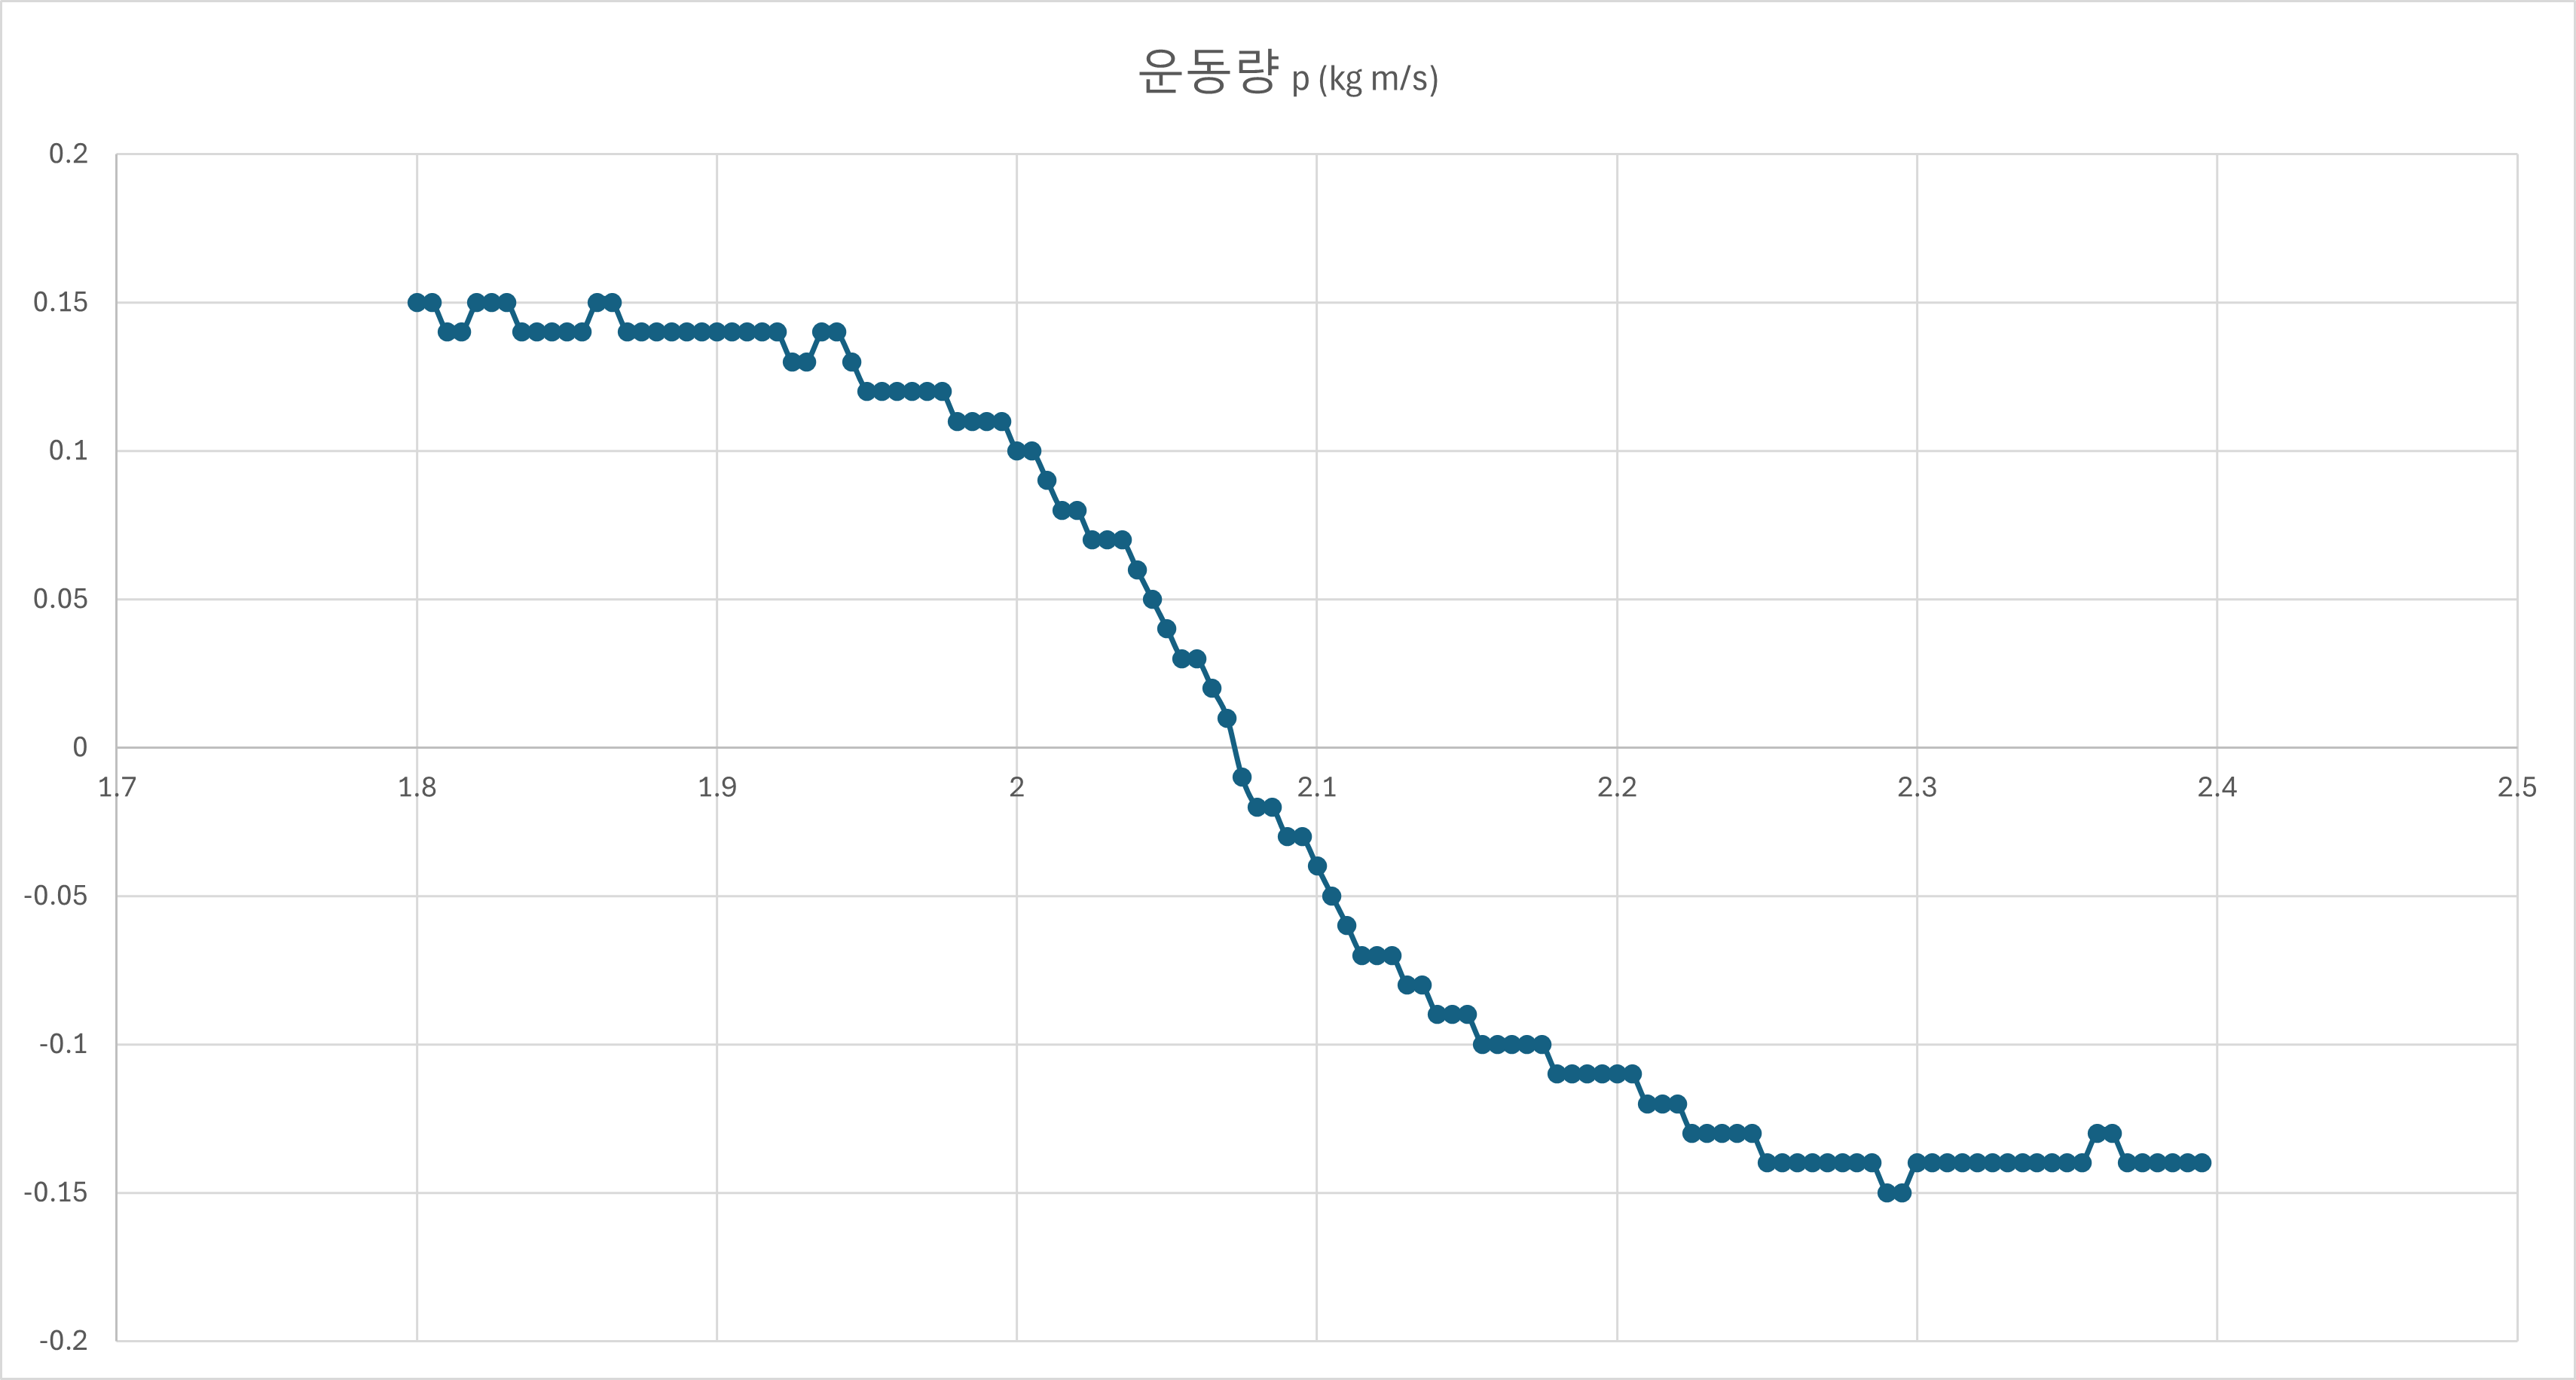
\includegraphics[width=6cm]{W11G6.png}
    \end{subfigure}
    \begin{subfigure}{0.4\textwidth}
        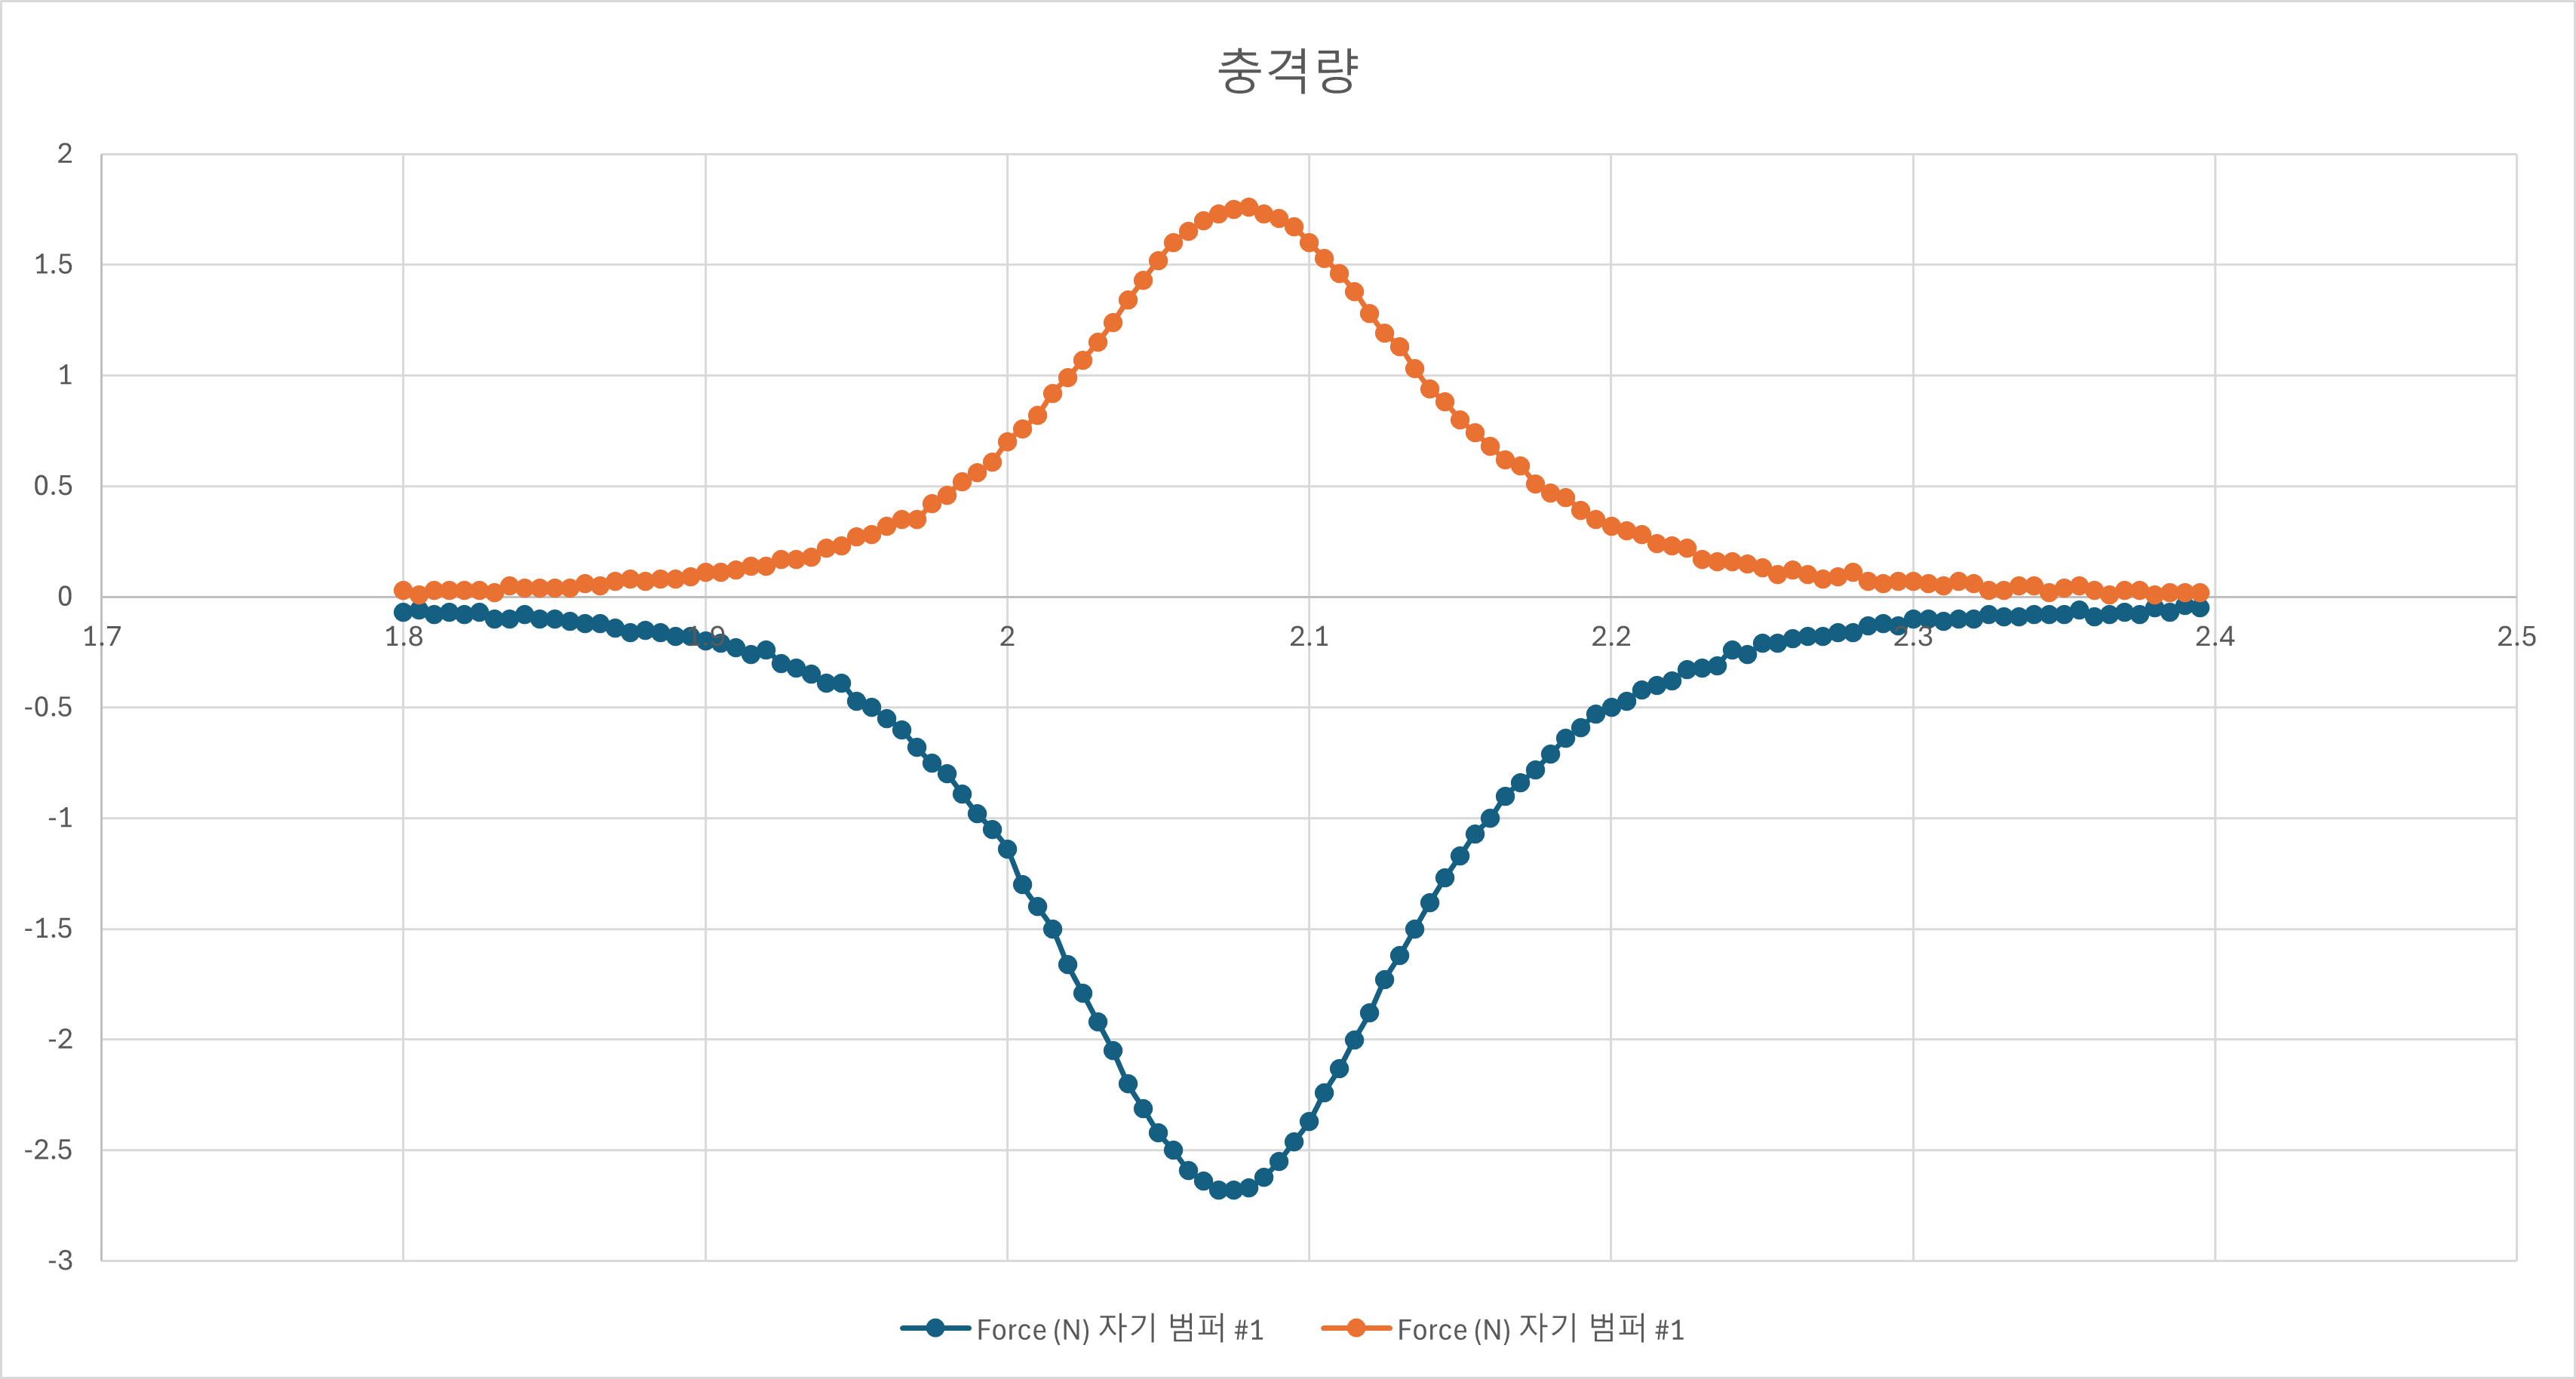
\includegraphics[width=6cm]{W11G7.png}
    \end{subfigure}
\end{figure}
자기적 반발력을 이용한 충돌실험

카트의 총 질량:$m=0.766kg$

\resizebox{15cm}{!}{
    \begin{tabular}{c|c|c|c|c|c|c}
        \hline
        \begin{tabular}{c}
            실험 \\
            횟수
        \end{tabular} &
        \begin{tabular}{c}
            충돌 전 속도 \\
            $v_i$ [m/s]
        \end{tabular} &
        \begin{tabular}{c}
            충돌 후 속도 \\
            $v_f$ [m/s]
        \end{tabular} &
        \begin{tabular}{c}
            운동량의 \\
            변화량 \\
            $\Delta p = m\left|v_f - v_i\right|$
        \end{tabular} &
        \begin{tabular}{c}
            충돌 지속시간 \\
            $\Delta t = \left|t_f - t_i\right|$
        \end{tabular} &
        \begin{tabular}{c}
            카트가 받은 충격량 \\
            $I$ [N$\cdot$s]
        \end{tabular} &
        \begin{tabular}{c}
            벽이 받은 충격량 \\
            $I'$ [N$\cdot$s]
        \end{tabular} \\
        \hline
        1 & $1.94\times10^{-1}$ & $-1.82\times10^{-1}$ & $2.88\times10^{-1}$ &
            $6.15\times10^{-1}$ & $2.88\times10^{-1}$ & $2.80\times10^{-1}$ \\
        \hline
        2 & $1.78\times10^{-1}$ & $-1.74\times10^{-1}$ & $2.70\times10^{-1}$ &
            $7.25\times10^{-1}$ & $2.70\times10^{-1}$ & $2.78\times10^{-1}$ \\
        \hline
        3 & $1.90\times10^{-1}$ & $-1.86\times10^{-1}$ & $2.88\times10^{-1}$ &
            $7.25\times10^{-1}$ & $2.88\times10^{-1}$ & $2.93\times10^{-1}$ \\
        \hline
        4 & $1.94\times10^{-1}$ & $-1.94\times10^{-1}$ & $2.97\times10^{-1}$ &
            $7.25\times10^{-1}$ & $2.97\times10^{-1}$ & $3.21\times10^{-1}$ \\
        \hline
        5 & $2.14\times10^{-1}$ & $-1.86\times10^{-1}$ & $3.06\times10^{-1}$ &
            $7.25\times10^{-1}$ & $3.06\times10^{-1}$ & $2.97\times10^{-1}$ \\
        \hline
        \multicolumn{3}{c|}{평균} & $2.90\times10^{-1}$ & $7.03\times10^{-1}$ &
            $2.90\times10^{-1}$ & $2.92\times10^{-1}$ \\
        \hline
    \end{tabular}
}
$$\textrm{상대오차}=\left|\textrm{운동량의 변화량}-\textrm{충격량}\right|/
    \textrm{충격량} \times 100 = 0.735\%$$
\subsection{실험2 용수철 반발력을 이용한 충돌실험}
충돌 전후의 운동량 변화와 충격량 구하기- 강한 스프링

\begin{figure}[h!]
    \centering
    \begin{subfigure}{0.4\textwidth}
        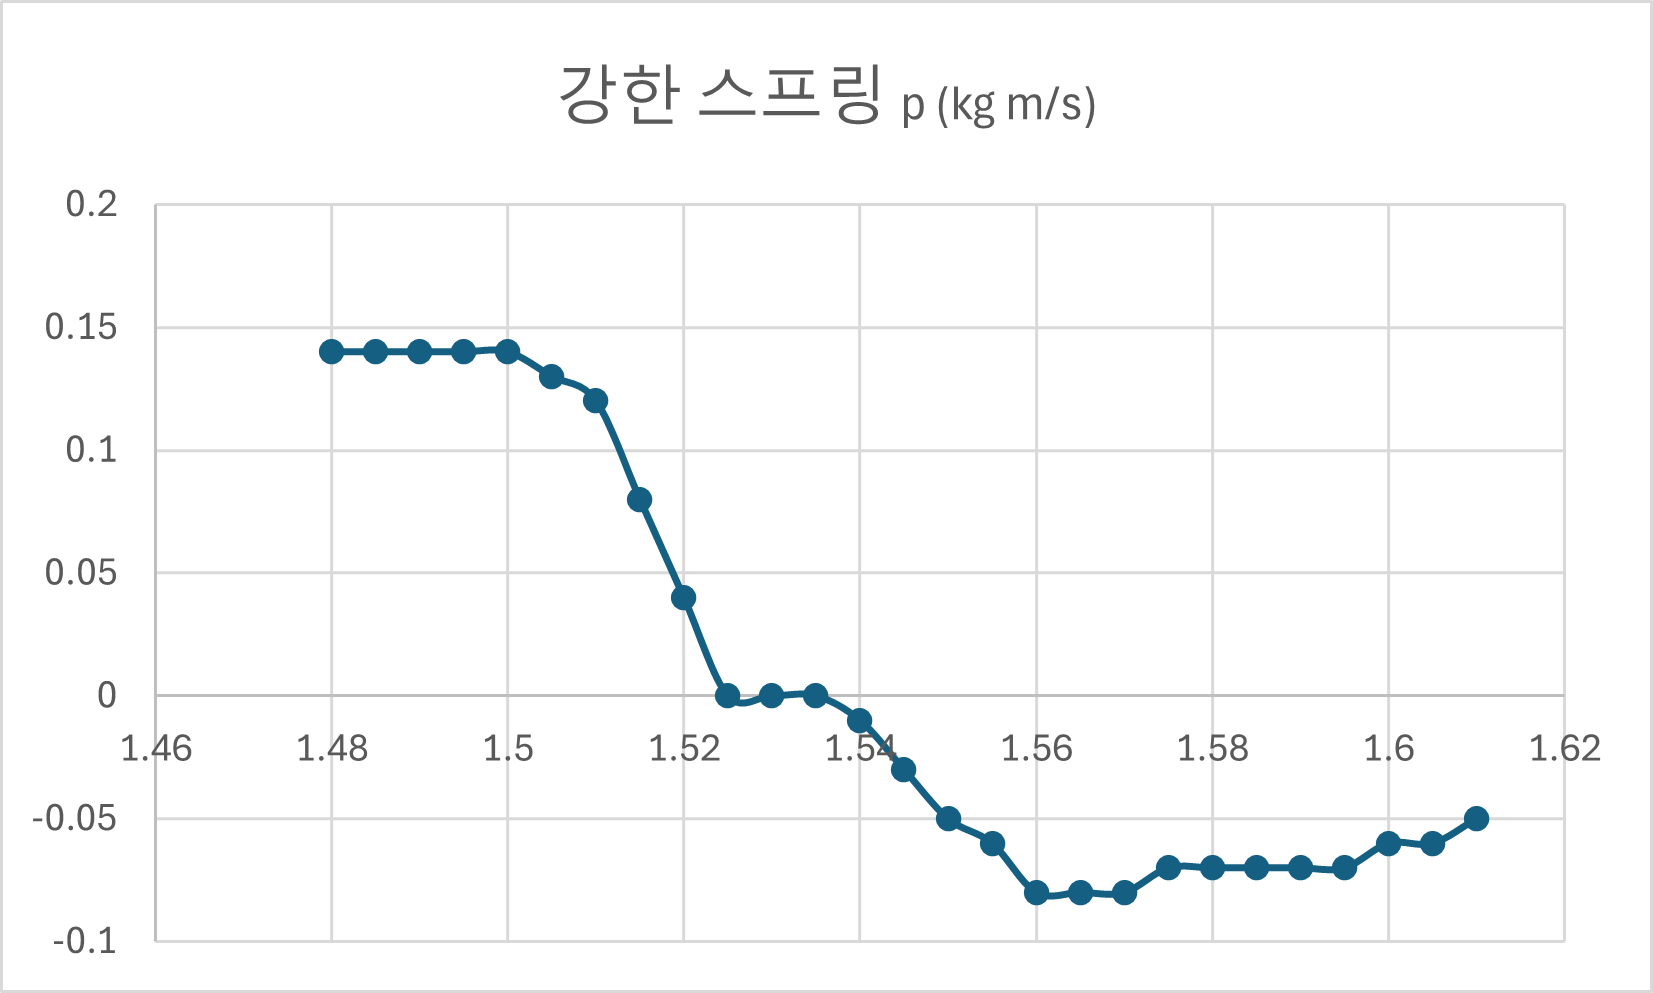
\includegraphics[width=6cm]{W11G8.png}
    \end{subfigure}
    \begin{subfigure}{0.4\textwidth}
        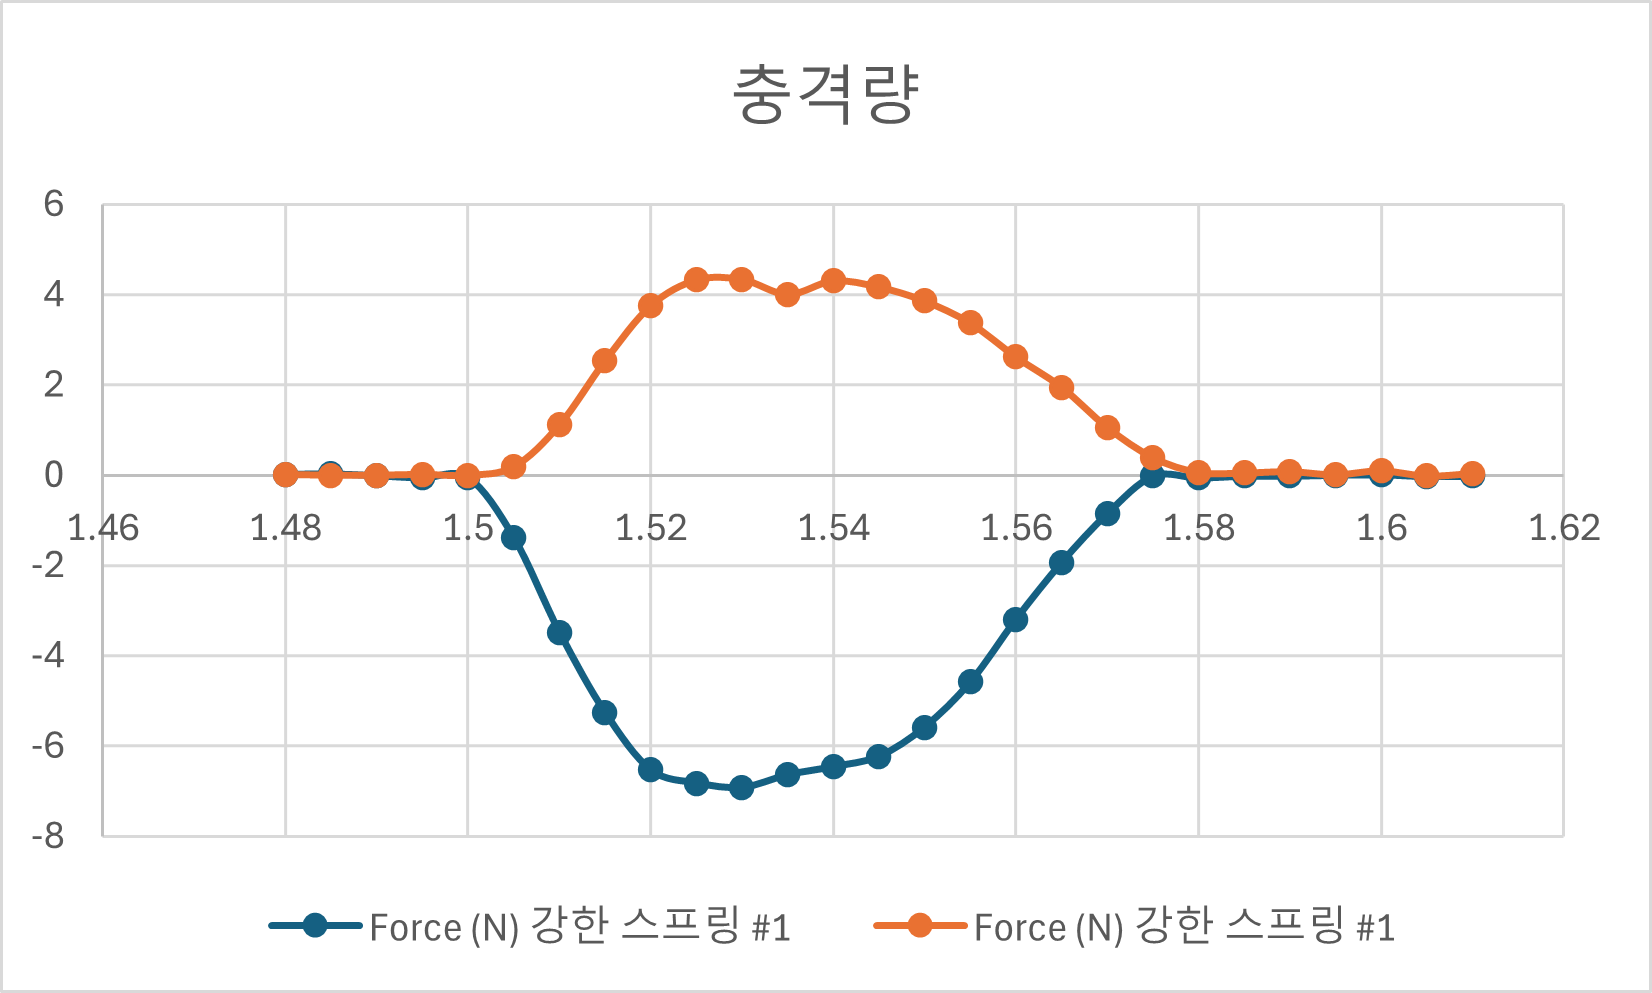
\includegraphics[width=6cm]{W11G9.png}
    \end{subfigure}
\end{figure}
강한 용수철 반발력을 이용한 충돌실험

카트의 총 질량:$m=0.748kg$

\resizebox{15cm}{!}{
    \begin{tabular}{c|c|c|c|c|c|c}
        \hline
        \begin{tabular}{c}
            실험 \\
            횟수
        \end{tabular} &
        \begin{tabular}{c}
            충돌 전 속도 \\
            $v_i$ [m/s]
        \end{tabular} &
        \begin{tabular}{c}
            충돌 후 속도 \\
            $v_f$ [m/s]
        \end{tabular} &
        \begin{tabular}{c}
            운동량의 \\
            변화량 \\
            $\Delta p = m\left|v_f - v_i\right|$
        \end{tabular} &
        \begin{tabular}{c}
            충돌 지속시간 \\
            $\Delta t = \left|t_f - t_i\right|$
        \end{tabular} &
        \begin{tabular}{c}
            카트가 받은 충격량 \\
            $I$ [N$\cdot$s]
        \end{tabular} &
        \begin{tabular}{c}
            벽이 받은 충격량 \\
            $I'$ [N$\cdot$s]
        \end{tabular} \\
        \hline
        1 & $1.86\times10^{-1}$ & $-7.28\times10^{-2}$ & $1.94\times10^{-1}$ &
            $1.35\times10^{-1}$ & $1.98\times10^{-1}$ & $2.12\times10^{-1}$ \\
        \hline
        2 & $1.94\times10^{-1}$ & $-0.93\times10^{-1}$ & $2.15\times10^{-1}$ &
            $1.05\times10^{-1}$ & $2.19\times10^{-1}$ & $2.15\times10^{-1}$ \\
        \hline
        3 & $2.02\times10^{-1}$ & $-1.05\times10^{-1}$ & $2.30\times10^{-1}$ &
            $0.95\times10^{-1}$ & $2.35\times10^{-1}$ & $2.34\times10^{-1}$ \\
        \hline
        4 & $1.94\times10^{-1}$ & $-0.93\times10^{-1}$ & $2.15\times10^{-1}$ &
            $0.10\times10^{-1}$ & $2.19\times10^{-1}$ & $2.18\times10^{-1}$ \\
        \hline
        5 & $2.02\times10^{-1}$ & $-1.05\times10^{-1}$ & $2.30\times10^{-1}$ &
            $1.05\times10^{-1}$ & $2.35\times10^{-1}$ & $2.28\times10^{-1}$ \\
        \hline
        \multicolumn{3}{c|}{평균} & $2.17\times10^{-1}$ & $1.08\times10^{-1}$ &
            $2.17\times10^{-1}$ & $2.21\times10^{-1}$ \\
        \hline
    \end{tabular}
}
$$\textrm{상대오차}=\left|\textrm{운동량의 변화량}-\textrm{충격량}\right|/
    \textrm{충격량} \times 100 = 2.23\%$$
\clearpage
충돌 전후의 운동량 변화와 충격량 구하기- 약한 스프링

\begin{figure}[h!]
    \centering
    \begin{subfigure}{0.4\textwidth}
        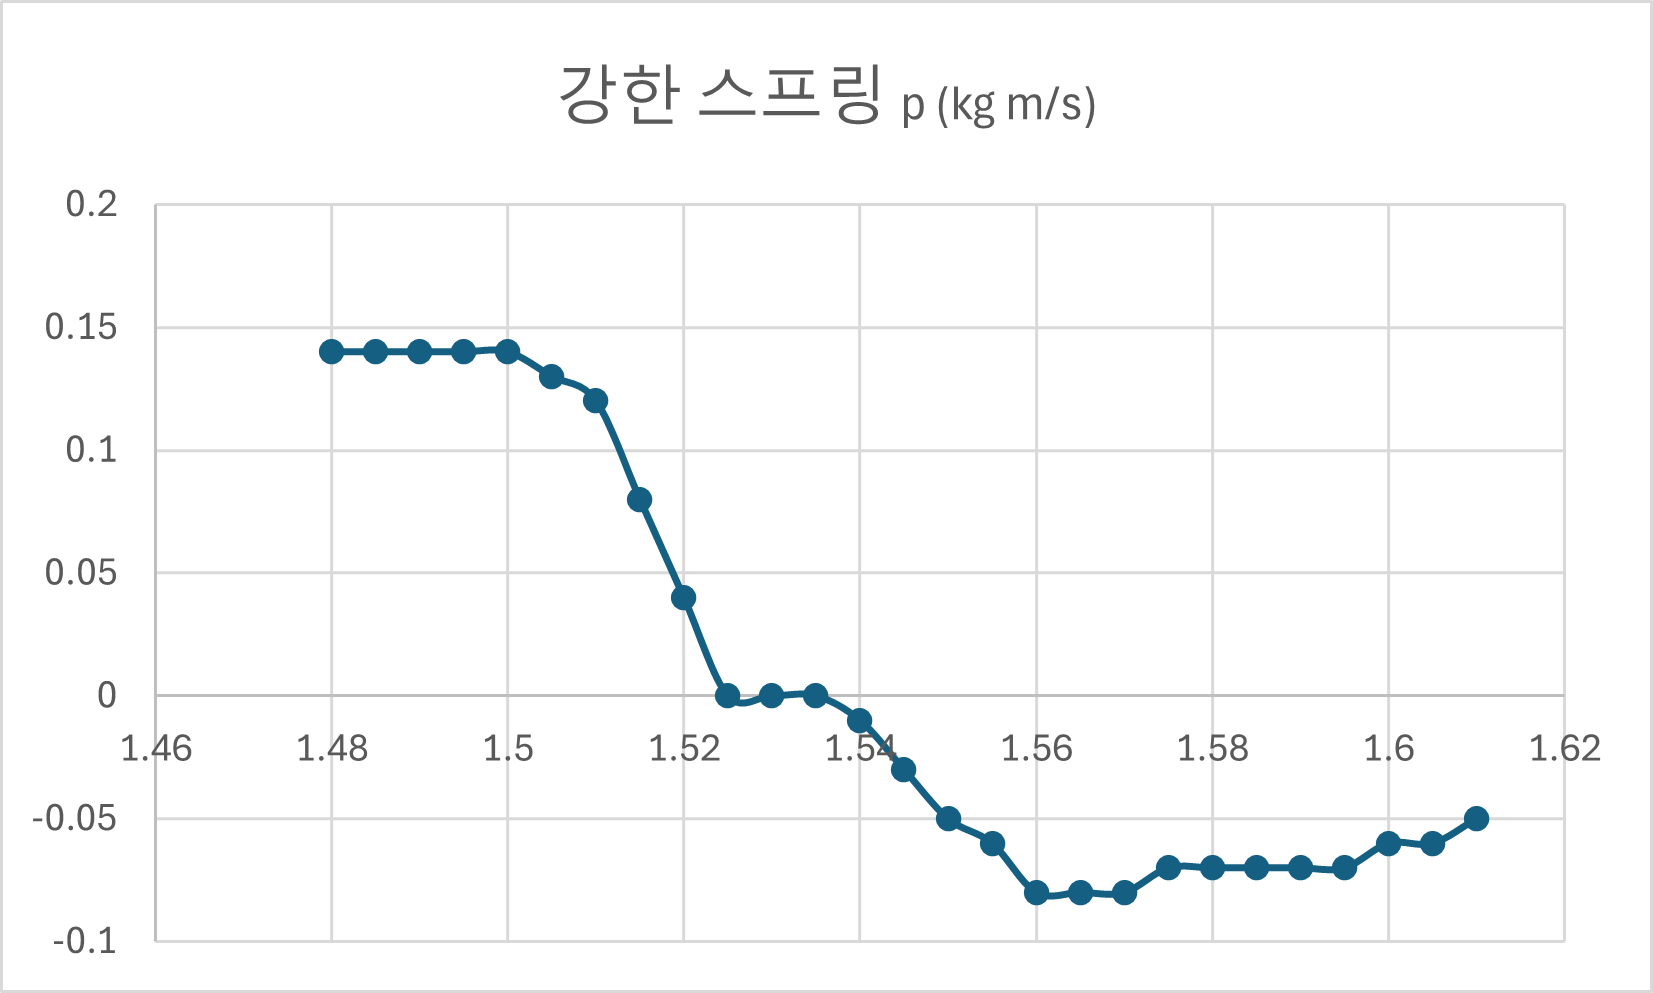
\includegraphics[width=6cm]{W11G8.png}
    \end{subfigure}
    \begin{subfigure}{0.4\textwidth}
        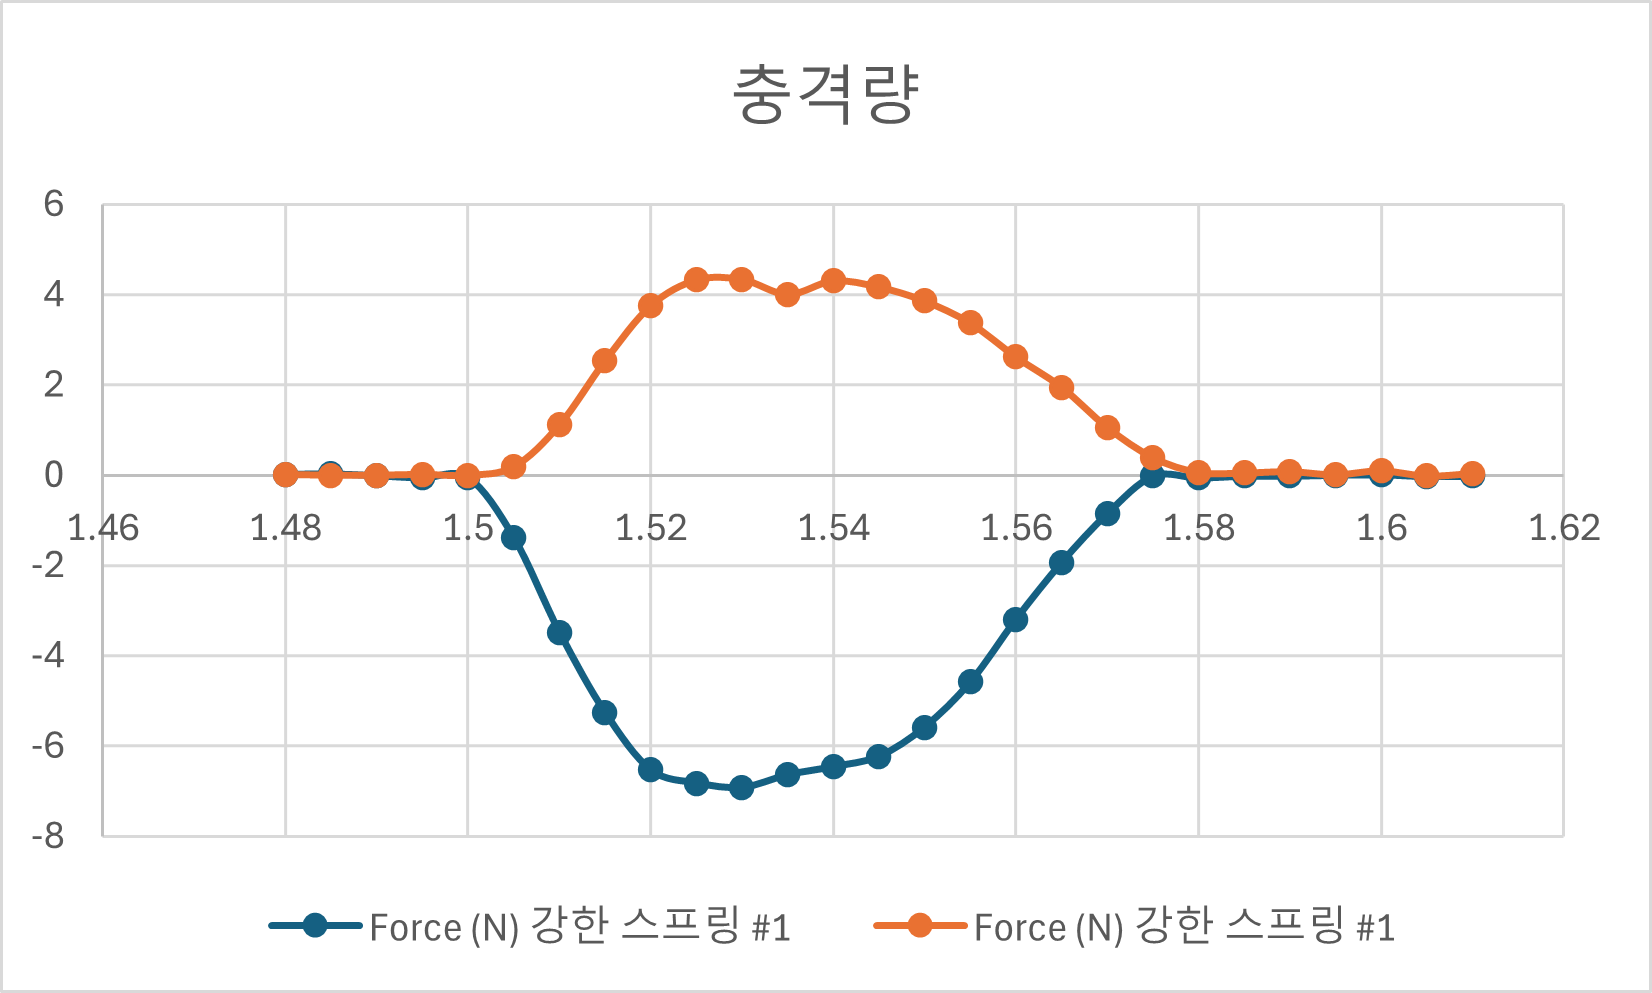
\includegraphics[width=6cm]{W11G9.png}
    \end{subfigure}
\end{figure}
약한 용수철 반발력을 이용한 충돌 실험

카트의 총 질량:$m=0.746kg$

\resizebox{15cm}{!}{
    \begin{tabular}{c|c|c|c|c|c|c}
        \hline
        \begin{tabular}{c}
            실험 \\
            횟수
        \end{tabular} &
        \begin{tabular}{c}
            충돌 전 속도 \\
            $v_i$ [m/s]
        \end{tabular} &
        \begin{tabular}{c}
            충돌 후 속도 \\
            $v_f$ [m/s]
        \end{tabular} &
        \begin{tabular}{c}
            운동량의 \\
            변화량 \\
            $\Delta p = m\left|v_f - v_i\right|$
        \end{tabular} &
        \begin{tabular}{c}
            충돌 지속시간 \\
            $\Delta t = \left|t_f - t_i\right|$
        \end{tabular} &
        \begin{tabular}{c}
            카트가 받은 충격량 \\
            $I$ [N$\cdot$s]
        \end{tabular} &
        \begin{tabular}{c}
            벽이 받은 충격량 \\
            $I'$ [N$\cdot$s]
        \end{tabular} \\
        \hline
        1 & $2.10\times10^{-1}$ & $-1.25\times10^{-2}$ & $2.56\times10^{-1}$ &
            $1.95\times10^{-1}$ & $2.50\times10^{-1}$ & $2.72\times10^{-1}$ \\
        \hline
        2 & $2.18\times10^{-1}$ & $-1.29\times10^{-1}$ & $2.65\times10^{-1}$ &
            $0.18\times10^{-1}$ & $2.59\times10^{-1}$ & $2.73\times10^{-1}$ \\
        \hline
        3 & $2.18\times10^{-1}$ & $-1.33\times10^{-1}$ & $2.68\times10^{-1}$ &
            $1.75\times10^{-1}$ & $2.62\times10^{-1}$ & $2.71\times10^{-1}$ \\
        \hline
        4 & $2.06\times10^{-1}$ & $-1.29\times10^{-1}$ & $2.56\times10^{-1}$ &
            $0.18\times10^{-1}$ & $2.50\times10^{-1}$ & $2.68\times10^{-1}$ \\
        \hline
        5 & $2.10\times10^{-1}$ & $-1.29\times10^{-1}$ & $2.59\times10^{-1}$ &
            $1.85\times10^{-1}$ & $2.53\times10^{-1}$ & $2.69\times10^{-1}$ \\
        \hline
        \multicolumn{3}{c|}{평균} & $2.54\times10^{-1}$ & $1.51\times10^{-1}$ &
            $2.54\times10^{-1}$ & $2.70\times10^{-1}$ \\
        \hline
    \end{tabular}
}
$$\textrm{상대오차}=\left|\textrm{운동량의 변화량}-\textrm{충격량}\right|/
    \textrm{충격량} \times 100 = 5.88\%$$
\subsection{‘운동량-충격량 정리’가 얼마나 잘 성립하는지 논하라. 위 실험 결과에
    서 운동량의 변화량과 충격량이 어떠한 관계가 있는지 ‘실험 이론’의 내
    용과 ‘실험 결과’를 토대로 비교하여 설명하라.}
카트가 받은 충격량과 벽이 받은 충격량의 상대 오차를 보면 0.735\%, 2.23\% 그리고
5.88\% 정도로 매우 작은 것을 알 수 있다. 이 때 카트가 받은 충격량은 운동량의 변화량과
같고, 이 값이 측정된 벽이 받은 충격량과의 관계로 미루어 보아, 잘 성립한다고 말 할 수
있다.
\subsection{단단한 물체와의 충돌과 부드러운 물체와의 충돌에서 충격량과 충돌시
    간을 비교하라.}
강한 스프링과 약한 스프링에서의 충격량을 보면 질량의 차이 정도의 값만 차이가 나고
충돌시간은 약한 스프링 쪽이 긴 것을 알 수 있다. 그러므로 약한 스프링에서의
$\Sigma\vec{F}$ 값은 평균적으로 강한 스프링에서의 그것과 비교하여 더 작을 것임을
알 수 있다.
\subsection{위의 비교를 응용하여, 차량의 에어백이 정면 층돌 시 탑승자가 다치는
    것을 어떻게 막을 수 있는지 설명하라}
에어백은 충돌시간을 늘림으로써 $I=\Sigma\vec{F}\Delta t$식에 따라 충격량이
유지되지만 시간이 늘어나게 만드면서 $\Sigma\vec{F}$값이 줄어들게 되어 탑승가가
느끼는 힘을 줄여서 탑승자의 부상을 예방한다.
\subsection{위의 실험 결과로 부터 충돌과정에서 작용 반작용이 성립하는지 설명해
    보라}
1,2,3실험 모두 다 카트의 충돌 시에 A카트가 역방향으로 가속된 것을 보면, 작용 반작용은
성립함을 알 수 있다.
\subsection{오차원인}
카트가 받은 충격량과 벽이 받은 충격량의 상대 오차를 보면 0.735\%, 2.23\% 그리고
5.88\%으로 점점 증가하는데, 아무래도 힘 센서의 오차값이 점점 누적된 것으로 보인다.
매 측정시마다 센서를 초기화했지만 이러한 오류가 생기는 것은 카트의 힘센서는
초기화했지만 고정 힘센서가 초기화가 되지 않았다거나 반대로 고정 힘센서는 초기화가
됐지만 카트 힘센서는 초기화가 안 됐을 수 있을 것 같다. 이를 방지하려면 매 측정시마다
영점조절 외에도 Calibration 탭에서 보정을 한다거나 식으로 초기화를 하고 값이 제대로
나오는지 힘센서끼리 연결하고 당겨보는 식으로 체크를 해 봐야 할 것 같다.
\subsection{실험을 통해 배우게 된 것}
\begin{itemize}
    \item 운동량의 변화량은 충격량과 같음을 알았다.
    \item 충돌 시간이 늘어나면 충격력이 줄어든다는 것을 알았다.
\end{itemize}
\subsection{실험원리의 실생활에서의 예}
\begin{itemize}
    \item 차량의 에어백
    \item 야구를 할 때에 나무배트보다 알루미늄 배트가 공이 더 멀리 날아간다.
\end{itemize}
\end{document}